% LyaMAPPO framework figure (CTDE) — submission-quality TikZ source.
% Mirrors docs/figures_paper/arch_lyamappo_framework.png (parameters verified
% against code: Actor 54-d, Critic 245-d, V=50, eta=0.5, reward weights
% 10/5/5/2/0.05, beta_task=0.5, GAE gamma=.99/lambda=.95, eps=.2, beta_e=.02).
% NOT compiled in the dev container (no LaTeX) — compile on Overleaf / TeX Live:
%   pdflatex arch_lyamappo_framework.tex
\documentclass[border=6pt]{standalone}
\usepackage{amsmath}
\usepackage{tikz}
\usetikzlibrary{positioning,arrows.meta,fit,backgrounds,calc}

\definecolor{cenv}{HTML}{3F6090}
\definecolor{cact}{HTML}{D62728}
\definecolor{clya}{HTML}{D97F0C}
\definecolor{ccri}{HTML}{2CA02C}
\definecolor{cppo}{HTML}{7E57C2}
\definecolor{cstar}{HTML}{B8860B}

\begin{document}
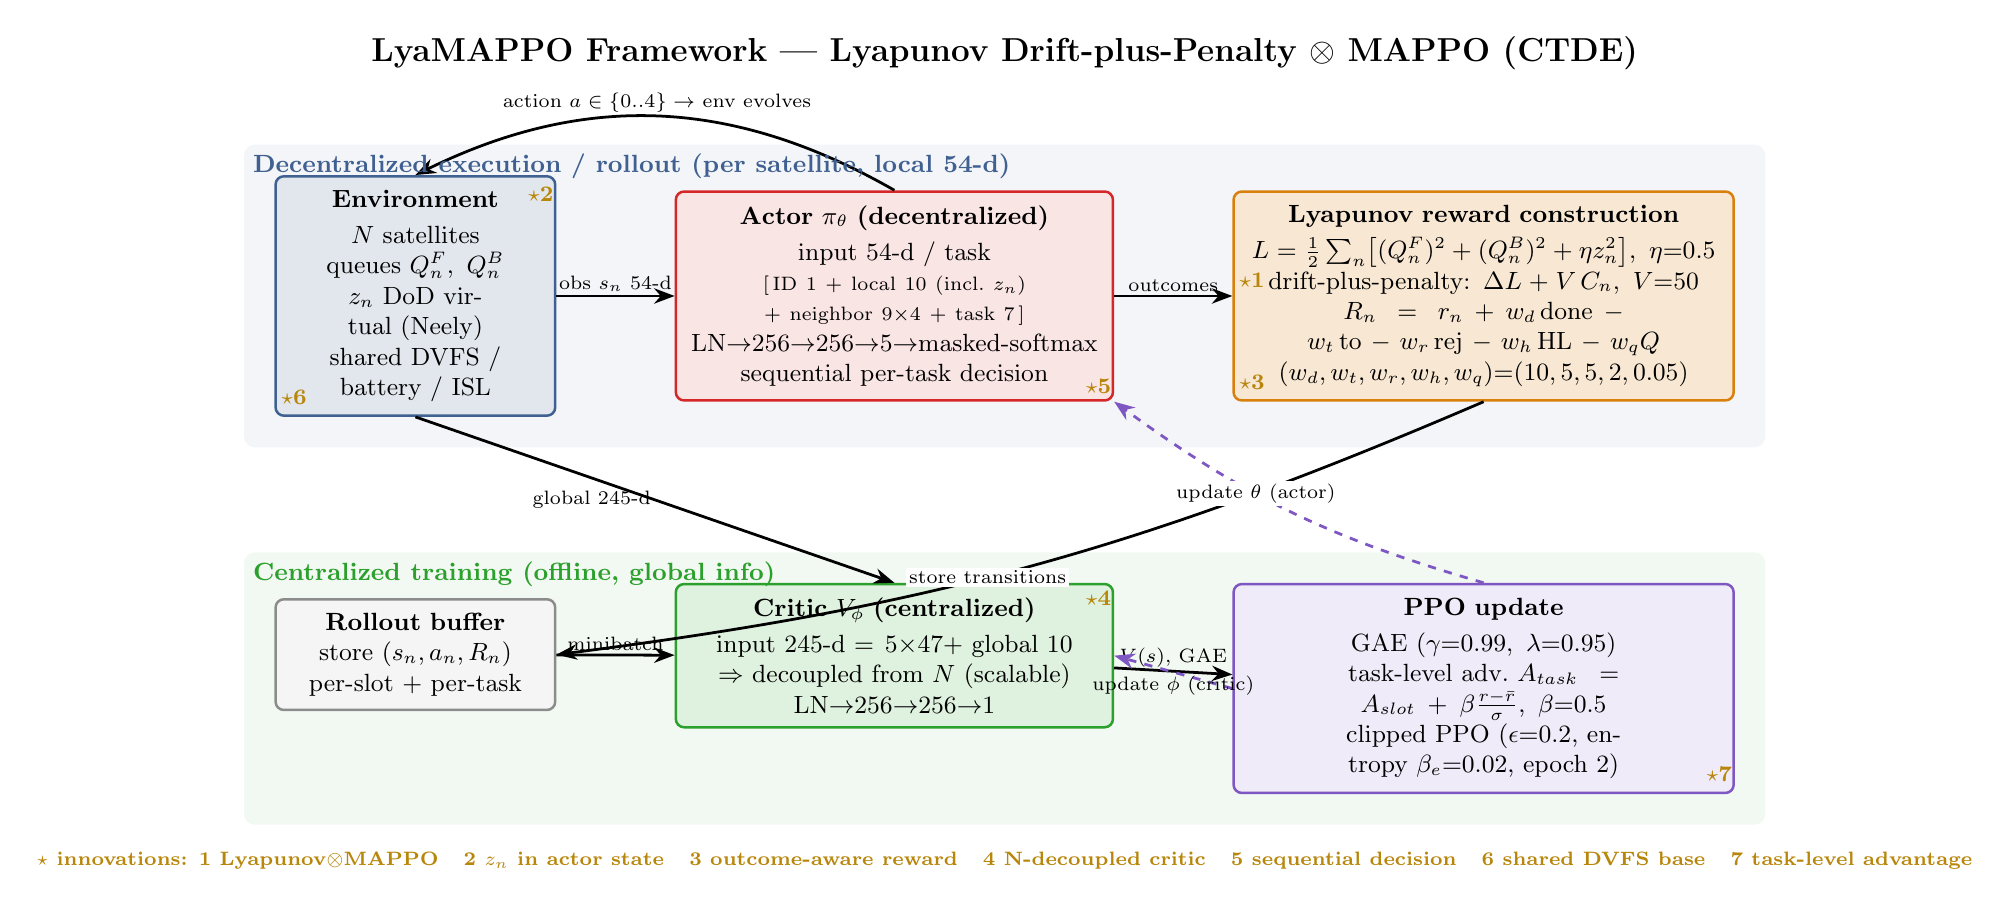
\begin{tikzpicture}[
  font=\small,
  >={Stealth[length=2.6mm]},
  box/.style={rounded corners=3pt, draw, line width=0.9pt, align=center,
              inner sep=5pt, text width=4.0cm},
  env/.style={box, fill=cenv!15, draw=cenv, text width=3.2cm},
  act/.style={box, fill=cact!12, draw=cact, text width=5.2cm},
  lya/.style={box, fill=clya!18, draw=clya, text width=6.0cm},
  cri/.style={box, fill=ccri!15, draw=ccri, text width=5.2cm},
  ppo/.style={box, fill=cppo!12, draw=cppo, text width=6.0cm},
  buf/.style={box, fill=black!4, draw=black!45, text width=3.2cm},
  flow/.style={->, line width=1.0pt},
  upd/.style={->, line width=1.0pt, dashed, draw=cppo},
  st/.style={text=cstar, font=\footnotesize\bfseries},
  note/.style={font=\scriptsize, inner sep=1pt},
]
% ---- top band: decentralized execution / rollout ----
\node[env] (env) {\textbf{Environment}\\[2pt]$N$ satellites\\ queues $Q^F_n,\ Q^B_n$\\ $z_n$ DoD virtual (Neely)\\ shared DVFS / battery / ISL};
\node[act, right=1.5cm of env] (act) {\textbf{Actor $\pi_\theta$ (decentralized)}\\[2pt] input 54-d / task\\ {\scriptsize[\,ID 1 + local 10 (incl.\ $z_n$) + neighbor $9{\times}4$ + task 7\,]}\\ LN$\to$256$\to$256$\to$5$\to$masked-softmax\\ sequential per-task decision};
\node[lya, right=1.5cm of act] (lya) {\textbf{Lyapunov reward construction}\\[2pt] $L=\tfrac12\sum_n\!\big[(Q^F_n)^2+(Q^B_n)^2+\eta z_n^2\big],\ \eta{=}0.5$\\ drift-plus-penalty: $\Delta L+V\,C_n,\ V{=}50$\\ $R_n=r_n+w_d\,\mathrm{done}-w_t\,\mathrm{to}-w_r\,\mathrm{rej}-w_h\,\mathrm{HL}-w_q Q$\\ $(w_d,w_t,w_r,w_h,w_q){=}(10,5,5,2,0.05)$};

% ---- bottom band: centralized training ----
\node[buf, below=2.3cm of env] (buf) {\textbf{Rollout buffer}\\ store $(s_n,a_n,R_n)$\\ per-slot + per-task};
\node[cri, below=2.3cm of act] (cri) {\textbf{Critic $V_\phi$ (centralized)}\\[2pt] input 245-d $=5{\times}47+$ global 10\\ $\Rightarrow$ decoupled from $N$ (scalable)\\ LN$\to$256$\to$256$\to$1};
\node[ppo, below=2.3cm of lya] (ppo) {\textbf{PPO update}\\[2pt] GAE ($\gamma{=}0.99,\ \lambda{=}0.95$)\\ task-level adv.\ $A_{task}=A_{slot}+\beta\tfrac{r-\bar r}{\sigma},\ \beta{=}0.5$\\ clipped PPO ($\epsilon{=}0.2$, entropy $\beta_e{=}0.02$, epoch 2)};

% ---- innovation stars ----
\node[st] at ($(env.north east)+(-0.2,-0.25)$) {$\star$2};
\node[st] at ($(env.south west)+(0.25,0.25)$) {$\star$6};
\node[st] at ($(act.south east)+(-0.2,0.2)$) {$\star$5};
\node[st] at ($(lya.west)+(0.25,0.2)$) {$\star$1};
\node[st] at ($(lya.south west)+(0.25,0.25)$) {$\star$3};
\node[st] at ($(cri.north east)+(-0.2,-0.2)$) {$\star$4};
\node[st] at ($(ppo.south east)+(-0.2,0.25)$) {$\star$7};

% ---- flows ----
\draw[flow] (env) -- node[note,above]{obs $s_n$ 54-d} (act);
\draw[flow] (act.north) to[bend right=28] node[note,above]{action $a\in\{0..4\}\to$ env evolves} (env.north);
\draw[flow] (act) -- node[note,above]{outcomes} (lya);
\draw[flow] (lya.south) to[bend left=8] node[note,pos=0.55,fill=white]{store transitions} (buf.east);
\draw[flow] (env.south) -- node[note,left]{global 245-d} (cri.north);
\draw[flow] (buf) -- node[note,above]{minibatch} (cri);
\draw[flow] (cri) -- node[note,above]{$V(s)$, GAE} (ppo);
\draw[upd] (ppo.north) to[bend left=10] node[note,pos=0.6,fill=white]{update $\theta$ (actor)} (act.south east);
\draw[upd] (ppo.west) -- node[note,below]{update $\phi$ (critic)} (cri.east);

% ---- CTDE bands (background) ----
\begin{scope}[on background layer]
  \node[fill=cenv!6, rounded corners=4pt, fit=(env)(act)(lya), inner sep=11pt] (top) {};
  \node[fill=ccri!6, rounded corners=4pt, fit=(buf)(cri)(ppo), inner sep=11pt] (bot) {};
\end{scope}
\node[anchor=north west, font=\small\bfseries, text=cenv] at (top.north west) {Decentralized execution / rollout (per satellite, local 54-d)};
\node[anchor=north west, font=\small\bfseries, text=ccri] at (bot.north west) {Centralized training (offline, global info)};
\node[font=\large\bfseries] at ($(top.north)+(0,1.15)$) {LyaMAPPO Framework — Lyapunov Drift-plus-Penalty $\otimes$ MAPPO (CTDE)};

% ---- innovation legend ----
\node[font=\scriptsize\bfseries, text=cstar, align=center] at ($(bot.south)+(0,-0.45)$)
  {$\star$ innovations: 1 Lyapunov$\otimes$MAPPO\quad 2 $z_n$ in actor state\quad 3 outcome-aware reward\quad 4 N-decoupled critic\quad 5 sequential decision\quad 6 shared DVFS base\quad 7 task-level advantage};
\end{tikzpicture}
\end{document}
